\documentclass[tikz,border=8pt]{standalone}
% Shared look for every TikZ diagram. Load with % Shared look for every TikZ diagram. Load with % Shared look for every TikZ diagram. Load with \input{../../tools/tikz-style.tex}
\usepackage[T1]{fontenc}
\usepackage{lmodern}
\renewcommand{\sfdefault}{lmr}  % diagrams use the same serif as the text
\usetikzlibrary{arrows.meta, positioning, shapes.geometric, calc, fit, backgrounds}
\definecolor{cblue}{HTML}{4C78A8}
\definecolor{corange}{HTML}{F58518}
\definecolor{cgreen}{HTML}{54A24B}
\definecolor{cred}{HTML}{E45756}
\definecolor{cpurple}{HTML}{B279A2}
\definecolor{cgrey}{HTML}{6B6B6B}
\tikzset{
  every picture/.style={font=\sffamily, line width=1.2pt},
  box/.style={draw=#1, fill=#1!12, rounded corners=4pt, align=center, inner sep=7pt, minimum height=1.1cm},
  box/.default=cgrey,
  arrow/.style={-{Stealth[length=3mm]}, draw=cgrey, line width=1.4pt},
  title/.style={font=\sffamily\bfseries\Large},
  note/.style={font=\sffamily\small, text=cgrey, align=center},
}
\AtBeginDocument{\hyphenpenalty=10000 \exhyphenpenalty=10000}

\usepackage[T1]{fontenc}
\usepackage{lmodern}
\renewcommand{\sfdefault}{lmr}  % diagrams use the same serif as the text
\usetikzlibrary{arrows.meta, positioning, shapes.geometric, calc, fit, backgrounds}
\definecolor{cblue}{HTML}{4C78A8}
\definecolor{corange}{HTML}{F58518}
\definecolor{cgreen}{HTML}{54A24B}
\definecolor{cred}{HTML}{E45756}
\definecolor{cpurple}{HTML}{B279A2}
\definecolor{cgrey}{HTML}{6B6B6B}
\tikzset{
  every picture/.style={font=\sffamily, line width=1.2pt},
  box/.style={draw=#1, fill=#1!12, rounded corners=4pt, align=center, inner sep=7pt, minimum height=1.1cm},
  box/.default=cgrey,
  arrow/.style={-{Stealth[length=3mm]}, draw=cgrey, line width=1.4pt},
  title/.style={font=\sffamily\bfseries\Large},
  note/.style={font=\sffamily\small, text=cgrey, align=center},
}
\AtBeginDocument{\hyphenpenalty=10000 \exhyphenpenalty=10000}

\usepackage[T1]{fontenc}
\usepackage{lmodern}
\renewcommand{\sfdefault}{lmr}  % diagrams use the same serif as the text
\usetikzlibrary{arrows.meta, positioning, shapes.geometric, calc, fit, backgrounds}
\definecolor{cblue}{HTML}{4C78A8}
\definecolor{corange}{HTML}{F58518}
\definecolor{cgreen}{HTML}{54A24B}
\definecolor{cred}{HTML}{E45756}
\definecolor{cpurple}{HTML}{B279A2}
\definecolor{cgrey}{HTML}{6B6B6B}
\tikzset{
  every picture/.style={font=\sffamily, line width=1.2pt},
  box/.style={draw=#1, fill=#1!12, rounded corners=4pt, align=center, inner sep=7pt, minimum height=1.1cm},
  box/.default=cgrey,
  arrow/.style={-{Stealth[length=3mm]}, draw=cgrey, line width=1.4pt},
  title/.style={font=\sffamily\bfseries\Large},
  note/.style={font=\sffamily\small, text=cgrey, align=center},
}
\AtBeginDocument{\hyphenpenalty=10000 \exhyphenpenalty=10000}

\newcommand{\cell}[4]{\node[draw=cgrey, line width=0.8pt, minimum size=0.95cm, fill=#4, font=\sffamily\large] at ({#1},{#2}) {#3};}
\begin{document}
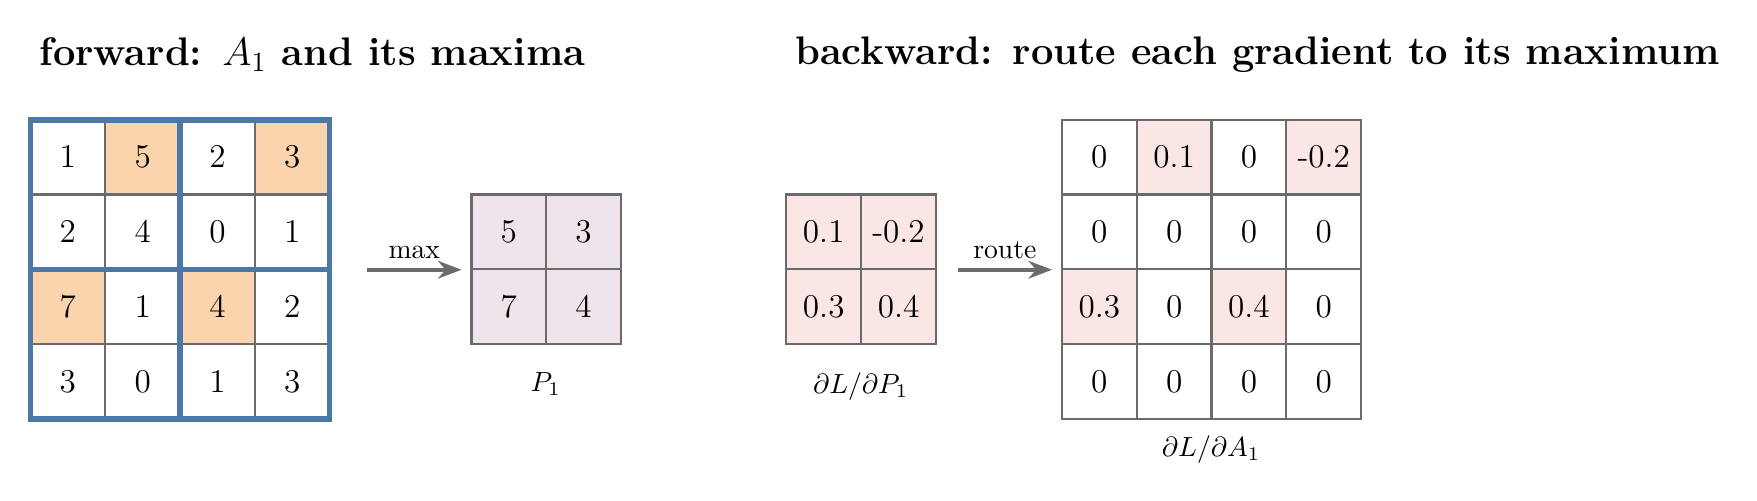
\begin{tikzpicture}
  % forward A1
  \node[title, anchor=west] at (-0.5,1.3) {forward: $A_1$ and its maxima};
  \foreach \v [count=\i from 0] in {1,5,2,3,2,4,0,1,7,1,4,2,3,0,1,3}{
    \pgfmathtruncatemacro{\r}{\i/4}\pgfmathtruncatemacro{\c}{mod(\i,4)}
    \edef\col{white}
    \ifnum\i=1 \edef\col{corange!35}\fi \ifnum\i=3 \edef\col{corange!35}\fi
    \ifnum\i=8 \edef\col{corange!35}\fi \ifnum\i=10 \edef\col{corange!35}\fi
    \cell{\c*0.95}{-\r*0.95}{\v}{\col}
  }
  \draw[cblue, line width=2pt] (-0.475,0.475) rectangle (1.425,-1.425);
  \draw[cblue, line width=2pt] (1.425,0.475) rectangle (3.325,-1.425);
  \draw[cblue, line width=2pt] (-0.475,-1.425) rectangle (1.425,-3.325);
  \draw[cblue, line width=2pt] (1.425,-1.425) rectangle (3.325,-3.325);
  \draw[arrow] (3.8,-1.43) -- (5.0,-1.43) node[midway, above] {max};
  \foreach \v [count=\i from 0] in {5,3,7,4}{
    \pgfmathtruncatemacro{\r}{\i/2}\pgfmathtruncatemacro{\c}{mod(\i,2)}
    \cell{5.6+\c*0.95}{-0.95-\r*0.95}{\v}{cpurple!20}
  }
  \node[below] at (6.07,-2.6) {$P_1$};
  % backward
  \begin{scope}[xshift=9.6cm]
  \node[title, anchor=west] at (-0.5,1.3) {backward: route each gradient to its maximum};
  \foreach \v [count=\i from 0] in {0.1,-0.2,0.3,0.4}{
    \pgfmathtruncatemacro{\r}{\i/2}\pgfmathtruncatemacro{\c}{mod(\i,2)}
    \cell{\c*0.95}{-0.95-\r*0.95}{\v}{cred!15}
  }
  \node[below] at (0.47,-2.6) {$\partial L/\partial P_1$};
  \draw[arrow] (1.7,-1.43) -- (2.9,-1.43) node[midway, above] {route};
  \foreach \v [count=\i from 0] in {0,0.1,0,-0.2,0,0,0,0,0.3,0,0.4,0,0,0,0,0}{
    \pgfmathtruncatemacro{\r}{\i/4}\pgfmathtruncatemacro{\c}{mod(\i,4)}
    \edef\col{white}
    \ifnum\i=1 \edef\col{cred!15}\fi \ifnum\i=3 \edef\col{cred!15}\fi
    \ifnum\i=8 \edef\col{cred!15}\fi \ifnum\i=10 \edef\col{cred!15}\fi
    \cell{3.5+\c*0.95}{-\r*0.95}{\v}{\col}
  }
  \node[below] at (4.92,-3.4) {$\partial L/\partial A_1$};
  \end{scope}
\end{tikzpicture}
\end{document}
